\documentclass{article}
\usepackage{amsmath}
\usepackage{amssymb}
\usepackage{graphicx}
\usepackage{hyperref}
\usepackage[version=4]{mhchem}

\title{Example 12}
\date{}

\begin{document}
\maketitle

Prove the angle bisector length formula\\
\(A D^{2}=A B \times A C-B D \times D C\)

Proof:
Extend \(A D\) to \(E\) such that \(\angle A B E=\angle A D C\).\\
\centering
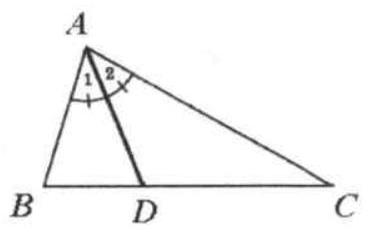
\includegraphics[width=\textwidth]{images/062.jpg}

We see that \(\triangle A B E \sim \triangle A D C\). Thus \(\frac{A B}{A D}=\frac{A E}{A C} \Rightarrow A B \times A C=A D \times A E\)\\
\centering
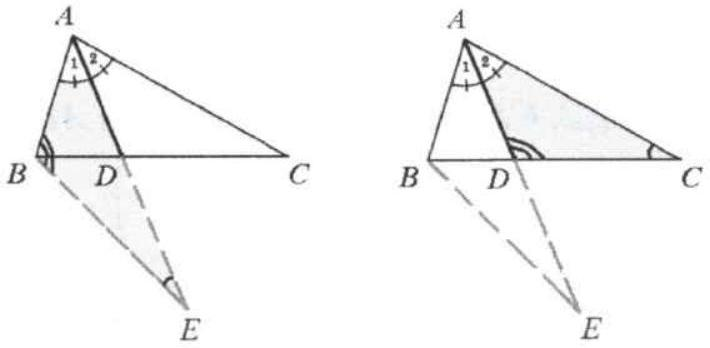
\includegraphics[width=\textwidth]{images/063(1).jpg}

We see that \(\triangle B D E \sim \triangle A D C\). Thus \(\frac{B D}{A D}=\frac{D E}{D C} \Rightarrow B D \times D C=A D \times D E\)\\
\centering
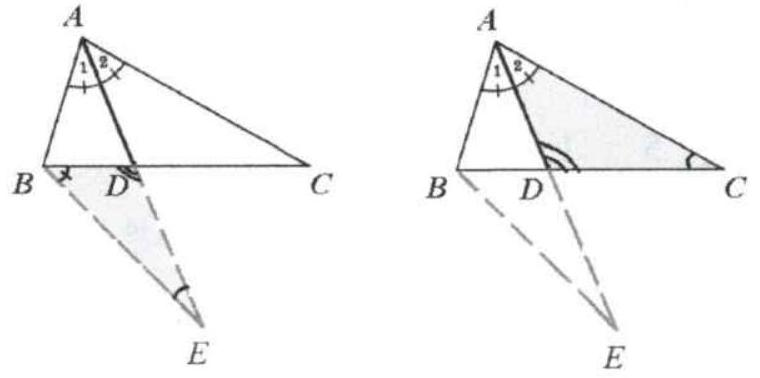
\includegraphics[width=\textwidth]{images/063.jpg}\\
(1) - (2): \(A B \times A C-B D \times D C=A D(A E-D E)=A D^{2}\). QED.

\end{document}
